\chapter[General introduction]{General introduction}
\label{chap1_generalintroduction}
 
\newpage 
 
\noindent Cancers of the colon and the rectum are the third most common type of cancer in the world, affecting over a million people annually \cite{c11}. In the general population, the lifetime risk of developing colorectal cancer is 5-6\% \cite{c12}. An increased risk of colorectal cancer has been observed for those with a history of colorectal cancer in one (2-fold) or 2 or more (4-fold) first degree family members \cite{c13}. Moreover, the personal risk of colorectal cancer nearly doubles if a colorectal adenoma, a benign established precursor of colorectal carcinoma \cite{c14,c15,c16,c17}, is diagnosed in a first-degree relative \cite{c13}. A personal history of colorectal adenomas also increases risk of developing recurrent colorectal carcinomas, particularly for those with a specific type of adenoma called villous adenoma (standardised incidence ratios (SIR) 2.1-5.0) \cite{c18,c19,c110}, adenomas 1 cm or larger (SIR 2.1-5.9) \cite{c18,c19,c110}, or multiple adenomas (SIR 1.3-4.8) \cite{
c110}. 
 
\noindent Furthermore, inheritance of cancer-associated genes strongly increases personal risk for colorectal cancer. Lynch syndrome is a well-known inherited cancer syndrome. Although Lynch syndrome is ``only'' responsible for up to 3\% of all colorectal cancers \cite{c111}, penetrance of colorectal cancer in Lynch syndrome is very high with 70-85\% developing colorectal cancer \cite{c112,c113,c114,c115,c116,c117}. Persons with Lynch syndrome inherit a pathogenic germline mutation in one of the mismatch repair (MMR) genes (\emph{MLH1}, \emph{MSH2}, \emph{MSH6}, and \emph{PMS2}), which results in microsatellite instability in tumours \cite{c118}. Microsatellites are short and repeated DNA sequences interspersed throughout the genome \cite{c119} that are vulnerable to mutation due to their repetitive nature \cite{c120}. During DNA replication, repeated sequences may shorten or lengthen, which causes ``instability'' and could also lead to protein inactivation \cite{c121}. Compared to the general population, 
individuals with Lynch 
syndrome have an increased risk for developing colorectal cancer to age 70, develop colorectal adenomas at a younger age, and have a higher lifetime risk for developing other cancers such as those in the endometrium, ovary, stomach, pancreas, small intestine, biliary system, and brain \cite{c113,c122,c123,c124,c125}. Figure \ref{figure1_1} depicts the risk of developing colorectal cancer  along a continuum of these clinical and genetic factors. 
 
% FIGURE 1 HERE 
\begin{figure} 
\begin{tikzpicture}[ ] 
%Declaration of styles 
\tikzstyle{box} = [rectangle, minimum width=3.5cm, minimum height=4.5cm, text centered, draw=black, text width = 3.2cm] %style for the boxes 
\tikzstyle{arr} = [single arrow, draw=black, text centered, minimum height = 13.15cm] %Style for the arrow 
 
%Nodes, the elements of the graphic 
\node [box] at (-4.05,0) {Low \quad\\ \quad\\ 3-5\% \quad\\ General population \quad\\ \quad\\ \quad\\ \quad\\ \quad\\}; 
\node [box] at (0,0) {Medium \quad\\ \quad\\  20-30\% \quad\\ Personal history \\ of CRA\\ Family history of CRC/CRA \quad\\ \quad\\}; 
\node [box] at (4.05,0) {High \quad\\ \quad\\  75-80\% \\ Lynch syndrome \quad\\ \quad\\ \quad\\ \quad\\ \quad\\}; 
\node [arr] at (0,-2.7) {\textbf{Colorectal cancer risk}}; 
\end{tikzpicture} 
\caption{Colorectal cancer risk along a continuum of clinical and genetic factors. \\ Abbreviations: CRA: colorectal adenomas; CRC: colorectal cancer.} 
\label{figure1_1} 
\end{figure} 
 
\noindent In addition to the cancer-related genes and a personal/family history of colorectal adenomas and carcinomas that predispose to an increased risk of colorectal cancer, dietary and lifestyle factors are also important in influencing the risk of developing colorectal cancer, possibly in combination with genetic susceptibility to these exposures due to specific variants in related metabolising genes \cite{c126,c127}. 
 
\section[]{Diet and colorectal cancer} %level 1 
\noindent The 2007 Second Expert Report by the World Cancer Research Fund/American Institute for Cancer Research (WCRF/AICR) estimates that roughly one-third, and even up to one-half in some countries, of all colorectal cancers could be prevented by regular physical activity, an avoidance of body fatness within the normal range of body weight, and proper food and nutrition \cite{c126}. More specifically, as part of the WCRF/AICR Continuous Update Project (CUP), the Colorectal Cancer 2011 Report judges that with respect to diet, there is convincing evidence that foods containing dietary fibre decrease risk of colorectal cancer, while red meat, processed meat, and alcoholic drinks (particularly in men) increase risk of developing colorectal cancer \cite{c127}. There is also suggestive evidence that non-starchy vegetables, fruits, and foods containing vitamin D could lower risk of colorectal cancer \cite{c127}. Micronutrients such as folate and other B vitamins may also impact risk of developing colorectal 
cancer \cite{c126,c127}. 
 
\noindent Folate is a water-soluble B vitamin found naturally in foods that include green leafy vegetables, fruits, nuts, dairy products, potatoes and other tubers, and meat products, particularly liver \cite{c128,c129}. In contrast to naturally occurring food folate, folic acid is the synthetic, chemically-stable form of folate and is used for food fortification and in dietary supplements \cite{c130}. Other related B vitamins include riboflavin (vitamin B2), pyridoxine (vitamin B6), and cobalamin (vitamin B12). In the Netherlands, the best food sources of vitamin B2 are milk and dairy products, while vitamin B6-rich foods include meat, fish, poultry, organ meats, nuts, and lentils; eggs, dairy products, and meat are excellent sources of vitamin B12 \cite{c129}. While not a B vitamin, the essential amino acid methionine is often included along with B vitamins in explorations between these nutrients and colorectal cancer risk. The reason behind this stems from the involvement of B vitamins and methionine in 
many biological reactions in one-carbon metabolism (OCM) that when disturbed, impact colorectal carcinogenesis \cite{c131,c132}. One-carbon metabolism will be more thoroughly discussed in later in this chapter in paragraph 2 of the section titled ``B vitamins, methionine, and DNA methylation''. Good dietary sources of methionine are animal products such as meat, eggs, and dairy. 
 
\noindent As noted above in paragraph 3, variants in metabolising genes such as those involved in one-carbon metabolism, may modify the relationships between dietary and lifestyle factors and risk of colorectal cancer. The enzyme methylenetetrahydrofolate reductase (MTHFR) plays a key role in OCM because its substrate, 5,10-mTHF, mediates one-carbon groups for pyrimidine synthesis, and its product supplies one-carbon groups for methylation of DNA and other molecules. The common C to T transition in the \textit{MTHFR} gene at nucleotide 677 results in an alanine to valine substitution, subsequently producing a thermolabile variant and reduced enzyme activity \cite{c133}. This functional SNP is possibly the most well-studied of all SNPs in OCM-related genes. Results from several meta-analyses indicate that by itself, the \textit{MTHFR} 677TT genotype has not been associated with risk of developing colorectal adenomas \cite{c134,c135} but has been associated with a decreased risk of colorectal cancer compared 
with the \textit{MTHFR} 677CC genotype \cite{c134,c135,c136}. In Lynch syndrome, the CT or TT genotype was associated with developing colorectal cancer at a later age (average age approximately 43 years) compared to those with the CC genotype (average age approximately 38 years) \cite{c137,c138}. 
 
\noindent While the \textit{MTHFR} 677TT genotype may not be associated with developing colorectal adenomas, it has been known to modify the associations between B vitamins and colorectal adenoma risk. Specifically, there has been a reduction in risk of colorectal adenomas for those with high folate intake and the TT genotype \cite{c139,c140,c141}; low folate intake in persons with the TT genotype has been associated with an increased risk of colorectal adenomas compared with CC individuals with high folate intake \cite{c141}. Likewise, the greatest risk reduction in colorectal cancer afforded by the \textit{MTHFR} 677TT genotype is for those with high blood folate or folate intake compared to CC or CT individuals with low folate \cite{c142,c143,c144,c145}. In some instances, low plasma folate in TT individuals increases the risk of developing colorectal cancer compared to those with high plasma folate and the CC or CT genotype \cite{c144}. 
 
\noindent The relationships between B vitamins and methionine with colorectal cancer are enormously complex. Not only are they are further complicated by genetic variation in OCM-associated metabolising genes but also by possible synergistic influences between the B vitamins with other nutrients in our diet and in combination with different food groups and may impact colorectal carcinogenesis differently depending on the timing of exposure (i.e. from healthy tissue to adenoma to carcinoma). 
 
\subsection{B vitamins, methionine, and colorectal carcinogenesis: evidence from epidemiological studies} % level 2 
 
\subsubsection{B-vitamins, methionine, and colorectal adenoma incidence and recurrence} % level 3 
\noindent The WCRF/AICR overview of data describing associations between colorectal adenomas and food, nutrition, and physical activity was published in 2006 \cite{c146}. Using data from two cohort studies, a meta-analysis of highest versus lowest category of dietary folate intake and incidence of colorectal adenomas found a non-significant inverse association between dietary folate intake and colorectal adenoma incidence (overall relative risk (RR) (95\%CI) of 0.85 (0.66-1.11)) \cite{c146}. Total folate intake (from diet and supplements) was inversely associated with colorectal adenomas risk (overall RR (95\%CI) of 0.75 (0.56-0.99)) \cite{c146}. 
 
\noindent For those who have been diagnosed with at least one colorectal adenoma, a meta-analysis of prospective cohort studies on dietary folate intake and colorectal adenoma recurrence showed a non-significant inverse association (overall RR (95\%CI) of 0.83 (0.60-1.14) \cite{c146}. Likewise, total folate intake was non-significantly inversely associated with colorectal adenoma recurrence (overall RR (95\%CI) of 0.78 (0.48-1.29)) \cite{c146}. Also increasing plasma folate concentrations decreased risk of adenoma recurrence (OR of 0.66 (95\%CI 0.46-0.97); P-trend=0.04) for high plasma folate \textit{vs}. low plasma folate) in a prospective cohort study \cite{c147}. Five randomised controlled trials have compared the recurrence of adenomas in patients receiving folic acid supplementation daily to those receiving placebo \cite{c148,c149,c150,c151,c152}. Two of the trials observed a benefit of folic acid supplementation \cite{c149,c151}, while two other trials found no effect \cite{c150,c152}. A large trial 
found a higher risk of having 3 or more adenomas or more advanced lesions ($\geq$ 25\% villous features, high-grade dysplasia, size $\geq$ 1 cm, or invasive cancer) with folic acid supplementation compared with placebo \cite{c148}. 
 
\noindent In individuals with no history of colorectal adenomas, two studies on vitamin B2 intake did not find an association with colorectal adenoma risk \cite{c153,c154}. One study did not find an association between plasma vitamin B2 and colorectal adenoma risk \cite{c155}. An inverse association between vitamin B2 intake and colorectal adenoma risk was observed in two studies \cite{c156,c157}, but only in one of these studies was the association significant \cite{c156}. Vitamin B6 intake is often \cite{c147,c153} but also not always \cite{c156} inversely associated with developing colorectal adenomas. There are also reports of inverse associations between the main circulating form of vitamin B6, PLP (pyridoxal 5'-phosphate), and colorectal adenoma risk \cite{c155,c158}. In the majority of studies, vitamin B12 status seems to be unassociated with first colorectal adenoma risk \cite{c155,c156,c158}. A meta-analysis of highest versus lowest category of methionine intake and colorectal adenoma incidence has 
been conducted using estimates from two cohort studies \cite{c146}. The pooled RR for colorectal adenoma incidence was 0.53 (0.25-1.11) \cite{c146}. In a cross-sectional study, plasma methionine was inversely associated with developing distal colorectal adenomas \cite{c155}. 
 
\noindent For those who have had at least one colorectal adenoma in their lifetime, vitamin B6 intake was inversely associated with risk of adenoma recurrence (OR of 0.65 (95\%CI 0.45-0.94); P-trend=0.03 for the highest quartile of intake \textit{vs}. the lowest) \cite{c147}. Likewise, vitamin B12 intake was inversely associated with risk of adenoma recurrence in a patients who had previously participated in an intervention study with wheat bran, but this association did not reach significance (for the highest quartile of intake \textit{vs}. lowest quartile OR of 0.74 (95\%CI 0.51-1.08); P-trend=0.14) \cite{c147}. One cohort study has reported an inverse but not significant association between methionine intake and recurrence of colorectal adenomas \cite{c147}. We are unaware of any studies on vitamin B2 intake and colorectal adenoma recurrence. Overall, foods containing folate, other B vitamins, and methionine may offer some protection against developing first or recurrent colorectal adenomas, but studies 
are not entirely consistent, particularly for vitamin B2, vitamin B12, and methionine, where the evidence is also more sparse. 
 
\subsubsection{B-vitamins, methionine, and colorectal cancer incidence} % level 3 
\noindent The earliest documented epidemiological observation of a link between folate intake and colorectal cancer was published in 1989 \cite{c159}. Decades of epidemiological research on folate, and more generally diet, and colorectal cancer have since followed. In 2005, Sanjoaquin and colleagues performed a meta-analysis of 7 cohort studies on folate intake and colorectal cancer risk and found an inverse association between dietary folate intake and colorectal cancer (overall RR for high \textit{vs}. low intake = 0.75; 95\%CI=0.64-0.89) \cite{c160}. These results have been corroborated by two meta-analyses \cite{c126,c161}, one of which was from the Second Expert Report (SER) by the WCRF/AICR that gave a summary effect estimate for the association between dietary folate intake and colorectal cancer of 0.84 (95\%CI 0.76-0.93) per 100 $\mu$g dietary folate/day \cite{c126}. Likewise, the most recent WCRF/AICR CUP summary estimates from meta-analyses for dietary folate intake and risk of colorectal cancer 
were also in the direction of decreased risk with increasing folate intake but did not reach statistical significance (summary effect estimate of 0.99 (95\%CI 0.93-1.05)) \cite{c127}. 
 
\noindent CUP summary relative risks from meta-analyses for serum/plasma folate (per 2 ng/mL) were also in the direction of decreased risk for colorectal cancer, colon cancer, and rectal cancer with increasing serum/plasma folate concentrations but were not significant (summary estimate of 0.97 (95\%CI 0.93-1.00) for colorectal cancer, 0.98 (0.85-1.14) for colon cancer, and 0.87 (0.70-1.09) for rectal cancer) \cite{c127}. Results from a pooled analysis of 5,720 colon cancer cases among 725,134 participants from 13 cohort studies showed a borderline significant decreased risk for those in the highest quintile of dietary folate intake compared with lowest group (pooled multivariate RR (95\%CI) of 0.92 (0.84-1.00)) \cite{c162}. Based on the current evidence, the WCRF/AICR has concluded that the evidence is too limited to draw conclusions about foods containing folate and risk of colorectal cancer. 
 
\noindent Regarding folic acid supplementation trials, a meta-analysis of randomised controlled trials has found no effect of folic acid supplementation on incidence of colorectal cancer \cite{c163}. Based on these results, folate may contribute a small protective effect against colorectal cancer, but because there are several inconsistencies results should be interpreted with prudence. 
 
\noindent Concerning the other B vitamins, there have been suggestions that higher vitamin B2 intakes \cite{c164} and higher concentrations of vitamin B2 in plasma/serum \cite{c165,c166} are associated with decreased risk of colorectal cancer, but to the best of our knowledge, no meta-analyses have been published thus far. For vitamin B6, the results of a meta-analysis that included nine prospective studies on vitamin B6 intake and four studies on PLP concentrations showed inverse associations between colorectal cancer risk and vitamin B6 intake (overall RR of 0.90 (0.75-1.07) for the highest \textit{vs} lowest category) and PLP concentrations (overall RR of  0.52 (95\% CI, 0.38-0.71 for the highest \textit{vs} lowest category) \cite{c167}. The relationships between vitamin B12 intake or plasma/serum vitamin B12 and colorectal cancer are less clear with most studies observing null associations \cite{c166,c168,c169,c170}. One study found an inverse association between methionine intake and colorectal cancer 
risk \cite{c164} while no associations were observed in two studies \cite{c168,c170}. Overall, these results taken together emphasise the need for more unambiguous evidence that describe associations between B vitamins and colorectal carcinogenesis. 

\section[]{Colorectal carcinogenesis: a continuum of genetic and epigenetic changes} % level 1 
\noindent Like all cancers, those that develop in the colon and rectum result from unregulated cellular growth. Over time, a stepwise accumulation of significant alterations, brought on by intrinsic or environmental factors \textendash~or a combination of both \textendash~modify the normal regulatory functions and dynamics of a cell \cite{c126}. As mentioned in paragraph 1 of this introduction, most precursor lesions of colorectal carcinomas are colorectal adenomas, and evolution from adenomas to carcinomas is termed the \textit{adenoma-carcinoma sequence} \cite{c14,c15,c16,c17}, during which tissues in the colon and rectum undergo histopathological changes with tissues becoming increasingly dysplastic \cite{c171}. The transition from normal epithelium to adenoma to carcinoma is accompanied by acquired molecular events that include genetic and epigenetic alterations \cite{c14,c172,c173}. 
 
\subsection{Genetic alterations during colorectal carcinogenesis} % level 2 
\noindent One of the earliest events of sporadic colorectal cancer progression that is required for colorectal adenoma formation is somatic bi-allelic inactivation of the tumour suppressor gene adenomatous polyposis coli (\textit{APC}) gene, leading to activation of the Wnt signalling pathway \cite{c174}. As well, Wnt signalling in some cancers may be activated by mutations in $\beta$-catenin. Wnt activation induces genes that include c-\textit{myc}, \textit{cyclin D1}, and \textit{PPAR-$\delta$} \cite{c175}. Transformation from early to late adenomas to carcinomas are likely due to mutations and/or loss of heterozygosity in the oncogene Kirsten-ras (\textit{KRAS}) \cite{c176}; mutations in the tumour suppressor gene \textit{p53} are proposed to be later events in the development of colorectal carcinomas \cite{c177}. The genetic basis of Lynch syndrome has been discussed in paragraph 2 of this chapter. Genetic changes in a cell during colorectal cancer progression are often accompanied by and interact with epigenetic 
modifications. 
 
\subsection{Epigenetic alterations during colorectal carcinogenesis} % level 2 
\noindent Epigenetics was first defined by C.H. Waddington as ``the causal interactions between genes and their products, which bring the phenotype into being'' \cite{c178}; the definition of epigenetics now encompasses the heritable changes in gene expression that occur independent of alterations in the DNA sequence \cite{c179}. Epigenetic processes include posttranslational modifications of histone proteins, nucleosome positioning along the DNA, and possibly the best-known of these processes, DNA methylation \cite{c173,c180}. 
 
\subsubsection{DNA methylation} % level 3 
\noindent DNA methylation occurs at the C-5 position of cytosine residues located in the CpG dinucleotide called CpG sites \cite{c181}. CpG sites, while under-represented in the genome, are found clustered together in C- and G-rich regions termed CpG islands, usually in the promoters or gene-regulating regions of genes. The remaining CpG sites are interspersed throughout the genome in transposable elements, repetitive sequences or other intronic regions of DNA. Typically in a healthy cell, most CpG islands are unmethylated and the associated genes subsequently expressed, while CpG sites are methylated \cite{c182,c183}. The methylation of CpG sites probably works to prevent chromosomal instability, translocations, and gene disruption caused by reactivation of transposable DNA sequences \cite{c184}. There are generally two different types of DNA methylation that can be described \textendash~gene-specific and global. 
 
\paragraph{Gene-specific DNA methylation} % level 4 
CpG islands in gene promoters or gene-regulating regions of genes are normally unmethylated in order to allow transcription of their corresponding genes. In cancer, these CpG islands may become more methylated (called gene-specific or promoter hypermethylation), which results in transcriptional silencing \cite{c185}. CpG island hypermethylation of promoters can affect genes involved in cell cycle, DNA repair, carcinogen metabolism, cell-cell interaction, apoptosis, and angiogenesis, all of which are related to carcinogenesis \cite{c182}. In colorectal carcinogenesis, CpG island promoter hypermethylation has been known to inactivate genes such as \textit{MLH1} (mismatch repair), \textit{p16\textsuperscript{INK4a}} (tumour suppressor), \textit{p14\textsuperscript{ARF}} (tumour suppressor), \textit{MGMT} (DNA repair), and \textit{RASSF1A} (tumour suppressor) \cite{c186,c187} in addition to numerous others. 
 
\paragraph{Global DNA methylation} % level 4 
In cancer, CpG sites that are distributed among the genome become less methylated, a process which is called global hypomethylation. Global hypomethylation is an early event in colorectal carcinogenesis \cite{c188,c189}. More explicitly, Fearon and Vogelstein's Genetic Model for Colorectal Tumorigenesis describes global DNA hypomethylation as an earlier event along the \textit{adenoma-carcinoma sequence} with gene-specific DNA methylation occurring later \cite{c14}. Because global DNA methylation is an earlier event in colorectal carcinogenesis and the aim of this thesis is to investigate relationships between B vitamins and DNA methylation along a continuum of risk for colorectal cancer that includes low-risk individuals, this thesis will focus on global DNA methylation. 
 
\paragraph{Measuring global DNA methylation in epidemiological studies} % level 4 
A plethora of methods have been developed to measure global DNA methylation, although the ``best'' method will depend on the number of samples, quality and quantity of available DNA, and desired coverage and resolution \cite{c190}. Chromatographic methods for measuring global DNA methylation allow for direct quantification of methylation. Following digestion of DNA into single strands, chromatographic methods directly measure the total number of 5-methyl cytosines and cytosines. Chromatography allows for direct quantification of DNA methylation but is time-consuming, costly and highly specialised equipment as well as large amounts of DNA are required, which can be cumbersome for large epidemiological studies \cite{c191}. As a possible alternative, in 2004, Yang and colleagues developed a PCR-based method to evaluate global DNA methylation by semi-quantitatively measuring methylation of long interspersed nuclear elements (LINEs) using bisulfite pyrosequencing \cite{c146}. LINEs are a variety of transposable 
elements. Transposable elements are mobile sequences of repetitive DNA that can migrate to different regions of the genome. There are two related LINE families, but the majority of genomic DNA is comprised of LINE-1 (18\%) \cite{c147}. Methylation of repetitive DNA elements such as LINE-1 is frequently used as a surrogate for global DNA methylation in epidemiological studies, including those where B vitamins are investigated as possible determinants of global DNA methylation \cite{c148,c149,c150,c151}. 
 
\section[]{B vitamins, methionine, and DNA methylation} % level 1 
\noindent As mentioned in paragraph 5, several B vitamins including folate play an essential role in one-carbon metabolism (OCM), where perturbations of B vitamins and methionine may have an effect on DNA methylation. One-carbon metabolism is a complex network of interconnected reactions involving a multitude of substrates, enzymes and cofactors \cite{c192} (see Figure \ref{focm}). Folate is a carrier of one-carbon units in OCM, where it plays a central role in DNA methylation, nucleotide synthesis, and maintaining DNA stability and repair \cite{c132,c193,c194,c195,c196}. 
 
\noindent In addition to folate, the B vitamins riboflavin (vitamin B2), pyridoxine (vitamin B6), and cobalamin (vitamin B12), and the essential amino acid methionine are also important in supporting efficient one-carbon metabolism \cite{c197}. Riboflavin in its coenzymatic form of flavin adenine dinucleotide (FAD) is essential for the enzyme methylenetetrahydrofolate reductase (MTHFR) in the irreversible reduction of 5,10-methylenetetrahydrofolate (5,10-methylene-THF) to 5-methyl-THF (5-mTHF) \cite{c198}. Vitamin B6 as pyridoxal 5'\ -phosphate is a coenzyme for serine hydroxymethyltransferase (SHMT) in the reversible conversion of tetrahydrofolate (THF) to 5,10-methylene-THF \cite{c199} while the remethylation of homocysteine to methionine by methionine synthase (MTR) and methionine synthase reductase (MTRR) with 5-methyl-THF as a methyl donor is dependent on cobalamin \cite{c1100,c1101}. Methionine is consequently metabolised to \textit{S}-adenosylmethionine (SAM), the universal methyl donor for over one 
hundred biological reactions including DNA methylation \cite{c1102}. High concentrations of homocysteine in blood are related to low blood concentrations of folate \cite{c1103}. Although B vitamins and methionine are involved in DNA synthesis and DNA stability and repair, which also influence colorectal cancer, this thesis focuses on the involvement of B vitamins on global DNA methylation. 
 
% FIGURE 2 HERE 
\begin{figure} 
\centering 
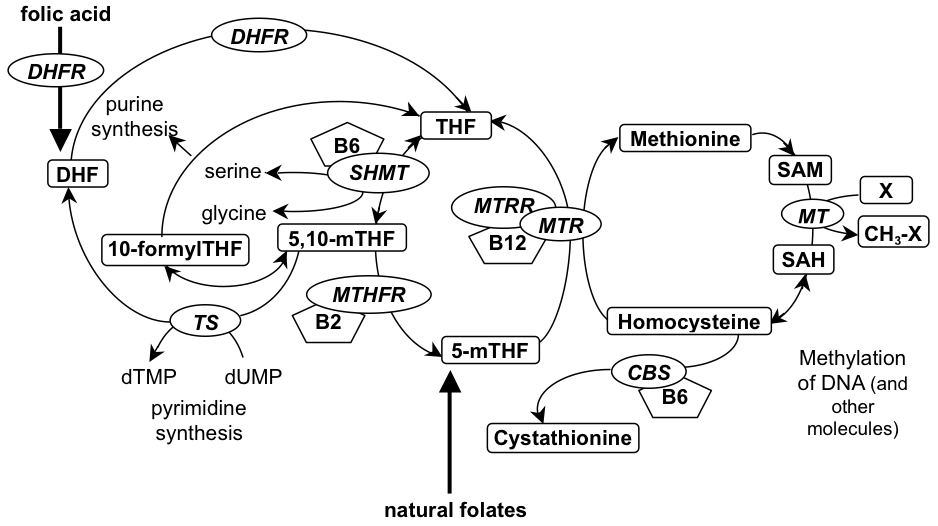
\includegraphics[width=0.85\textwidth]{ocm_xls5.jpg} 
\caption{Folate-mediated one-carbon metabolism. Abbreviations: DHF: dihydrofolate; DHFR: dihydrofolate reductase; THF: tetrahydrofolate; SHMT: serine hydroxymethyltransferase; 10-formylTHF: 10-formyltetrahydrofolate; 5,10-mTHF: 5,10-methylenetetrahydrofolate; 5-mTHF: 5-methyltetrahydrofolate; MTHFR: methylenetetrahydrofolate reductase; MTRR: methionine synthase reductase; MTR: methionine synthase; CBS: cystathionine $\beta$-synthase; MT: methyltransferase; SAM: \emph{S}-adenosylmethionine; SAH: \emph{S}-adenosylhomocysteine} 
\label{focm} 
\end{figure} 
 
 
\section[]{B vitamins and leukocyte DNA methylation: \\ evidence from epidemiological studies} % level 1 
\noindent The role of B vitamins along the continuum of colorectal carcinogenesis is not straightforward, and may depend on a plethora of factors, such as inefficient OCM, personal history of colorectal adenomas, a family history of colorectal adenomas and carcinomas, and inherited mutations in cancer-associated genes. Likewise, the impact of B vitamins on DNA methylation could be moderated by the presence or absence of these factors. 
 
\noindent The relationships between B vitamins and DNA methylation have been studied in normal colorectal tissues \cite{c1104,c1105}, colorectal adenomas \cite{c1106}, and colorectal carcinomas \cite{c1107,c1108}. With this in mind, the intent of this thesis is to better understand the influence of B vitamins on leukocyte global DNA methylation of populations differing in risk for colorectal cancer. 
 
\subsection{Low risk population} % level 2 
\noindent There have been two relatively short-term (12 weeks) randomised placebo-controlled trials investigating the effects of folic acid supplementation on leukocyte global DNA methylation in populations at low-risk for colorectal cancer \cite{c1109,c1110}. At the end of 12 weeks, neither trial found an effect of 1.2 mg \cite{c1109} nor 2 mg \cite{c1110} daily folic acid supplementation on global DNA methylation. A possible explanation for these null results could be the short duration of folic acid supplementation and the use of supraphysiological doses of folic acid. Two cross-sectional studies, one in urban commuters in the United States and the other in older Brazilians (aged 60-88 years) have reported that neither intake of natural folates nor dietary folate equivalents was associated with leukocyte LINE-1 methylation \cite{c1111}, nor global DNA methylation \cite{c1112}. A third cross-sectional study observed that higher dietary folate intake was associated with lower global DNA methylation in Japanese women \
cite{c1113}. Geographical differences, food fortification, different dietary habits, and baseline folate concentrations are some reasons that could possibly account for these dissimilar results. Similarly, plasma folate has been unassociated with leukocyte global methylation in a cross-sectional analysis \cite{c1114} in contrast to two other controlled folate intake studies in women, where leukocyte global DNA methylation decreased following folate depletion \cite{c1115,c1116}. In one of these studies, DNA hypomethylation was reversed following folate repletion \cite{c1115}, but not in the other \cite{c1116}. This is likely due to the study population, comprised exclusively of elderly women, where stabilisation of DNA methylation following folate depletion could be delayed, resulting also in a slower response to folate repletion. 

\noindent Three cross-sectional studies have examined relationships between intake of other B vitamins and leukocyte DNA methylation \cite{c1111,c1112,c1113}. One study found a weak negative correlation between vitamin B6 intake and global DNA methylation (Spearman $\rho$ of -0.18, P=0.04) \cite{c1112}. Vitamin B12 intake was not related to global DNA methylation, and vitamin B2 was not investigated \cite{c1112}. On the other hand, intake of vitamins B2, B6, and B12 were not associated with leukocyte global DNA methylation in an urban American population \cite{c1111}, nor in Japanese women \cite{c1113}. 
 
\subsection{High risk population} % level 2 
\noindent The association between B vitamins and global DNA methylation has been investigated in colorectal adenoma patients. These associations have not yet been explored in a Lynch syndrome population. In colorectal adenoma patients, the effects of folic acid supplementation on global DNA methylation were investigated \cite{c1117}. After 10 weeks of daily supplementation with 400 $\mu$g folic acid, leukocyte global DNA methylation increased 31\% (95\%CI 16-47\%; p=0.05 \textit{vs}. placebo). Here, the dose and duration of folic acid supplementation was lower and shorter, respectively than in trials with low-risk participants, but there was an effect on global DNA methylation, which was measured using the same method as in the other low-risk trials. Baseline red blood folate also appeared to be similar between the three populations. Drawing firm conclusions is not possible based on one study, but it is possible to speculate that folic acid has a different effect on DNA methylation depending on which phase during 
carcinogenesis it is given. Additionally, genetic variation in OCM-related genes, such \textit{MTHFR}, could modify the relationships between B vitamins and methionine with DNA methylation. 
 
\section[]{B vitamins and DNA methylation: interactions with \emph{MTHFR} C677T} % level 1 
\noindent Main effects of the \textit{MTHFR} C677T genotype on global DNA methylation have been explored in several studies. In low risk populations, there has been no difference in leukocyte global DNA methylation levels between genotypes \cite{c1112,c1113,c1114}. However, the C677T polymorphism in this gene may modify associations between plasma folate and global DNA methylation and LINE-1 DNA methylation. 
 
\subsection{Low risk population} % level 2 
\noindent Two studies have suggested that leukocyte DNA is hypomethylated in persons with low folate status and homozygous for the TT genotype \cite{c133,c1118}. In a folate depletion-repletion study, women with the TT genotype had a greater in increase in leukocyte DNA global DNA methylation following folate repletion compared with the CC genotype \cite{c1119}. A similar folate depletion-repletion study found lower levels of leukocyte DNA methylation in women with the TT genotype following repletion compared with CC or CT women \cite{c1120}. The slow response in DNA methylation levels to folate repletion has been partly attributed to a slow turnover of whole-body folate pools \cite{c1121}. On the whole, there seem to be interactions between folate intake and \textit{MTHFR} C677T in a low-risk population. The largest variation in global DNA methylation (i.e. greatest increase and decrease of global DNA methylation) by folate intake appear to be most clear in those with the \textit{MTHFR} 677TT genotype. 
 
\subsection*{High risk population} % level 2 
\noindent In very high risk populations, data on B vitamin-colorectal cancer relationships are not yet available. There was no information about dietary information nor DNA methylation from the two studies that investigated the main effects of the \textit{MTHFR} C677T single nucleotide polymorphism on colorectal cancer risk in persons with Lynch syndrome \cite{c137,c138}. 
 
\section[]{Rationale and Outline of this Thesis} % level 1 
\noindent The main purpose of the studies presented in this thesis is to improve our knowledge about the associations between B vitamin and methionine status and leukocyte global DNA methylation in populations with differential risk for developing colorectal cancer. Figure \ref{figure3} is an illustration of the clinical, genetic, and nutritional factors that influence differential risk for colorectal cancer along a continuum as outlined in this thesis according to each chapter. Given that DNA methylation is one of the major mechanisms linking B vitamins and other nutritional factors to colorectal cancer, \textbf{Chapter 2} is a review that summarises the impact of nutrition on DNA methylation in different cancer sites as explored in epidemiological studies. 
 
\noindent In order to study the relationships between B vitamin status and global DNA methylation in different risk groups, we use data from four study populations differing in colorectal cancer risk, as shown in Figure \ref{figure3}. Contributions from these studies begin in \textbf{Chapter 3} where the relationship between plasma folate and leukocyte LINE-1 methylation in a low risk population was explored. A study detailing the effects of folic acid supplementation on leukocyte global DNA methylation in individuals with moderately elevated homocysteine is presented in \textbf{Chapter 4}. Moving further along the risk scale for colorectal cancer, \textbf{Chapter 5} investigates the associations between plasma B vitamins and methionine, and LINE-1 methylation in colorectal adenoma patients; additional effect modification by number of lifetime colorectal adenomas was also explored. Associations between dietary B vitamin and methionine intake and risk of colorectal tumours in Lynch Syndrome individuals are 
studied in \textbf{Chapter 6}. This thesis concludes (\textbf{Chapter 7}) with a discussion of the results from all our studies. Recommendations for future research and public health implications are additionally considered. 
 
% FIGURE 3 HERE 
\begin{figure} 
\begin{tikzpicture}[ ] 
%Declaration of styles 
	\tikzstyle{box} = [rectangle, minimum width=3.0cm, minimum height=4.3cm, text centered, draw=black, text width = 2.7cm] %style for the boxes 
	\tikzstyle{arr} = [single arrow, draw=black, text centered, minimum height = 13.15cm] %Style for the arrow 
%Nodes, the elements of the graphic 
	\node [box] at (-4.85,0) {Low \quad\\ \quad\\ 3-5\% \quad\\ General population \quad\\ \quad\\ \quad\\ \quad\\Chapter 3}; 
	\node [box] at (-1.70,0) {Medium \quad\\ \quad\\ 4.5-7.5\%\quad\\ Decreased folate\\concentrations \quad\\ \quad\\ \quad\\ \quad\\Chapter 4}; 
    	\node [box] at (1.45,0) {High \quad\\ \quad\\ 20-30\% \\ Personal history \\ of CRA \\ Family history of CRC/CRA \quad\\ \quad\\Chapter 5}; 
    	\node [box] at (4.60,0) {Very high \quad\\ \quad\\ 75-80\% \quad\\ Lynch syndrome \quad\\ \quad\\ \quad\\ \quad\\ \quad\\Chapter 6}; 
    	\node [arr] at (0,-2.8) {\textbf{Colorectal cancer risk}}; 
\end{tikzpicture} 
\caption{Colorectal cancer risk along a continuum of clinical, genetic, and nutritional factors according to the chapters of this thesis.} 
\label{figure3} 
\end{figure} 
 
\renewcommand{\bibname}{References} 
\begin{thebibliography}{12} 
	\bibitem{c11}	Ferlay J, Shin HR, Bray F, Forman D, Mathers C, Parkin DM. GLOBOCAN 2008 v2.0, Cancer Incidence and Mortality Worldwide: IARC CancerBase No. 10 [Internet]. Lyon, France: International Agency for Research on Cancer; 2010. Available from: http://globocan.iarc.fr, accessed on 21/08/2013. 
	\bibitem{c12}	Siegel R, Naishadham D, Jemal A. Cancer statistics, 2013. CA: a cancer journal for clinicians. 2013 Jan;63(1):11-30. 
	\bibitem{c13}	Butterworth AS, Higgins JP, Pharoah P. Relative and absolute risk of colorectal cancer for individuals with a family history: a meta-analysis. Eur J Cancer. 2006 Jan;42(2):216-27. 
	\bibitem{c14}	Fearon ER, Vogelstein B. A genetic model for colorectal tumorigenesis. Cell. 1990 Jun 1;61(5):759-67. 
	\bibitem{c15}	Morson BC. Precancerous lesions of the colon and rectum. Classification and controversial issues. JAMA. 1962 Feb 3;179:316-21. 
	\bibitem{c16}	Chen CD, Yen MF, Wang WM, Wong JM, Chen TH. A case-cohort study for the disease natural history of adenoma-carcinoma and de novo carcinoma and surveillance of colon and rectum after polypectomy: implication for efficacy of colonoscopy. British Journal of Cancer. 2003 Jun 16;88(12):1866-73. 
	\bibitem{c17}	Hill MJ, Morson BC, Bussey HJ. Aetiology of adenoma--carcinoma sequence in large bowel. Lancet. 1978 Feb 4;1(8058):245-7. 
	\bibitem{c18}	Loeve F, van Ballegooijen M, Boer R, Kuipers EJ, Habbema JD. Colorectal cancer risk in adenoma patients: a nation-wide study. International Journal of Cancer. 2004 Aug 10;111(1):147-51. 
	\bibitem{c19}	Simons BD, Morrison AS, Lev R, Verhoek-Oftedahl W. Relationship of polyps to cancer of the large intestine. Journal of the National Cancer Institute. 1992 Jun 17;84(12):962-6. 
	\bibitem{c110}	Atkin WS, Morson BC, Cuzick J. Long-term risk of colorectal cancer after excision of rectosigmoid adenomas. The New England Journal of Medicine. 1992 Mar 5;326(10):658-62. 
	\bibitem{c111}	de la Chapelle A. The incidence of Lynch syndrome. Familial cancer. 2005;4(3):233-7. 
	\bibitem{c112}	Aarnio M, Mecklin JP, Aaltonen LA, Nystrom-Lahti M, Jarvinen HJ. Life-time risk of different cancers in hereditary non-polyposis colorectal cancer (HNPCC) syndrome. International Journal of Cancer. 1995 Dec 20;64(6):430-3. 
	\bibitem{c113}	Aarnio M, Sankila R, Pukkala E, Salovaara R, Aaltonen LA, de la Chapelle A, et al. Cancer risk in mutation carriers of DNA-mismatch-repair genes. International Journal of Cancer. 1999 Apr 12;81(2):214-8. 
	\bibitem{c114}	Weitz J, Koch M, Debus J, Hohler T, Galle PR, Buchler MW. Colorectal cancer. Lancet. 2005 Jan 8-14;365(9454):153-65. 
	\bibitem{c115}	Dunlop MG, Farrington SM, Carothers AD, Wyllie AH, Sharp L, Burn J, et al. Cancer risk associated with germline DNA mismatch repair gene mutations. Human molecular genetics. 1997 Jan;6(1):105-10. 
	\bibitem{c116}	Watson P, Lynch HT. Cancer risk in mismatch repair gene mutation carriers. Familial cancer. 2001;1(1):57-60. 
	\bibitem{c117}	Vasen HF, Wijnen JT, Menko FH, Kleibeuker JH, Taal BG, Griffioen G, et al. Cancer risk in families with hereditary nonpolyposis colorectal cancer diagnosed by mutation analysis. Gastroenterology. 1996 Apr;110(4):1020-7. 
	\bibitem{c118}	Vasen HF, Moslein G, Alonso A, Bernstein I, Bertario L, Blanco I, et al. Guidelines for the clinical management of Lynch syndrome (hereditary non-polyposis cancer). Journal of Medical Genetics. 2007 Jun;44(6):353-62. 
	\bibitem{c119}	Richard GF, Kerrest A, Dujon B. Comparative genomics and molecular dynamics of DNA repeats in eukaryotes. Microbiol Mol Biol Rev. 2008 Dec;72(4):686-727. 
	\bibitem{c120}	Koole W, Schafer HS, Agami R, van Haaften G, Tijsterman M. A versatile microsatellite instability reporter system in human cells. Nucleic acids research. 2013 Jul 16. 
	\bibitem{c121}	Lynch HT, de la Chapelle A. Hereditary colorectal cancer. The New England Journal of Medicine. 2003 Mar 6;348(10):919-32. 
	\bibitem{c122}	Half EE, Bresalier RS. Clinical management of hereditary colorectal cancer syndromes. Current opinion in gastroenterology. 2004 Jan;20(1):32-42. 
	\bibitem{c123}	Hampel H, Stephens JA, Pukkala E, Sankila R, Aaltonen LA, Mecklin JP, et al. Cancer risk in hereditary nonpolyposis colorectal cancer syndrome: later age of onset. Gastroenterology. 2005 Aug;129(2):415-21. 
	\bibitem{c124}	Watson P, Lynch HT. The tumor spectrum in HNPCC. Anticancer Research. 1994 Jul-Aug;14(4B):1635-9. 
	\bibitem{c125}	Kastrinos F, Mukherjee B, Tayob N, Wang F, Sparr J, Raymond VM, et al. Risk of pancreatic cancer in families with Lynch syndrome. JAMA. 2009 Oct 28;302(16):1790-5. 
	\bibitem{c126}	World Cancer Research Fund/American Institute for Cancer Research. Food, Nutrition, Physical Activity, and the Prevention of Cancer: a Global Perspective. Washington DC: AICR, 2007. 
	\bibitem{c127}	World Cancer Research Fund/American Institute for Cancer Research. Continuous Update Project Report. Food, Nutrition, Physical Activity, and the Prevention of Colorectal Cancer. 2011. 
	\bibitem{c128}	Konings EJ, Roomans HH, Dorant E, Goldbohm RA, Saris WH, van den Brandt PA. Folate intake of the Dutch population according to newly established liquid chromatography data for foods. The American Journal of Clinical Nutrition. 2001 Apr;73(4):765-76. 
	\bibitem{c129}	van Rossum CTM, Fransen HP, Verkaik-Kloosterman J, Buurma-Rethans EJM, Ock MC. Dutch National Food Consumption Survey 2007-2010. Bilthoven: National Institute for Public Health and the Environment; 2011. Report No.: 350050006/2011. 
	\bibitem{c130}	Winkels RM, Brouwer IA, Siebelink E, Katan MB, Verhoef P. Bioavailability of food folates is 80\% of that of folic acid. The American Journal of Clinical Nutrition. 2007 Feb;85(2):465-73. 
	\bibitem{c131}	Little J, Sharp L, Duthie S, Narayanan S. Colon cancer and genetic variation in folate metabolism: the clinical bottom line. The Journal of Nutrition. 2003 Nov;133(11 Suppl 1):3758S-66S. 
	\bibitem{c132}	Ulrich CM. Nutrigenetics in cancer research--folate metabolism and colorectal cancer. The Journal of Nutrition. 2005 Nov;135(11):2698-702. 
	\bibitem{c133}	Friso S, Choi SW, Girelli D, Mason JB, Dolnikowski GG, Bagley PJ, et al. A common mutation in the 5,10-methylenetetrahydrofolate reductase gene affects genomic DNA methylation through an interaction with folate status. Proceedings of the National Academy of Sciences of the United States of America. 2002 Apr 16;99(8):5606-11. 
	\bibitem{c134}	Huang Y, Han S, Li Y, Mao Y, Xie Y. Different roles of MTHFR C677T and A1298C polymorphisms in colorectal adenoma and colorectal cancer: a meta-analysis. Journal of human genetics. 2007;52(1):73-85. 
	\bibitem{c135}	Zacho J, Yazdanyar S, Bojesen SE, Tybjaerg-Hansen A, Nordestgaard BG. Hyperhomocysteinemia, methylenetetrahydrofolate reductase c.677C>T polymorphism and risk of cancer: cross-sectional and prospective studies and meta-analyses of 75,000 cases and 93,000 controls. International Journal of Cancer. 2011 Feb 1;128(3):644-52. 
	\bibitem{c136}	Taioli E, Garza MA, Ahn YO, Bishop DT, Bost J, Budai B, et al. Meta- and pooled analyses of the methylenetetrahydrofolate reductase (MTHFR) C677T polymorphism and colorectal cancer: a HuGE-GSEC review. American Journal of Epidemiology. 2009 Nov 15;170(10):1207-21. 
	\bibitem{c137}	Pande M, Chen J, Amos CI, Lynch PM, Broaddus R, Frazier ML. Influence of methylenetetrahydrofolate reductase gene polymorphisms C677T and A1298C on age-associated risk for colorectal cancer in a caucasian lynch syndrome population. Cancer Epidemiol Biomarkers Prev. 2007 Sep;16(9):1753-9. 
	\bibitem{c138}	Reeves SG, Meldrum C, Groombridge C, Spigelman AD, Suchy J, Kurzawski G, et al. MTHFR 677 C>T and 1298 A>C polymorphisms and the age of onset of colorectal cancer in hereditary nonpolyposis colorectal cancer. Eur J Hum Genet. 2009 May;17(5):629-35. 
	\bibitem{c139}	Ulvik A, Evensen ET, Lien EA, Hoff G, Vollset SE, Majak BM, et al. Smoking, folate and methylenetetrahydrofolate reductase status as interactive determinants of adenomatous and hyperplastic polyps of colorectum. American Journal of Medical Genetics. 2001 Jul 1;101(3):246-54. 
	\bibitem{c140}	Marugame T, Tsuji E, Kiyohara C, Eguchi H, Oda T, Shinchi K, et al. Relation of plasma folate and methylenetetrahydrofolate reductase C677T polymorphism to colorectal adenomas. International Journal of Epidemiology. 2003 Feb;32(1):64-6. 
	\bibitem{c141}	Ulrich CM, Kampman E, Bigler J, Schwartz SM, Chen C, Bostick R, et al. Colorectal adenomas and the C677T MTHFR polymorphism: evidence for gene-environment interaction? Cancer Epidemiol Biomarkers Prev. 1999 Aug;8(8):659-68. 
	\bibitem{c142}	Le Marchand L, Wilkens LR, Kolonel LN, Henderson BE. The MTHFR C677T polymorphism and colorectal cancer: the multiethnic cohort study. Cancer Epidemiol Biomarkers Prev. 2005 May;14(5):1198-203. 
	\bibitem{c143}	Chen J, Giovannucci E, Kelsey K, Rimm EB, Stampfer MJ, Colditz GA, et al. A methylenetetrahydrofolate reductase polymorphism and the risk of colorectal cancer. Cancer research. 1996 Nov 1;56(21):4862-4. 
	\bibitem{c144}	Ma J, Stampfer MJ, Giovannucci E, Artigas C, Hunter DJ, Fuchs C, et al. Methylenetetrahydrofolate reductase polymorphism, dietary interactions, and risk of colorectal cancer. Cancer research. 1997 Mar 15;57(6):1098-102. 
	\bibitem{c145}	Slattery ML, Potter JD, Samowitz W, Schaffer D, Leppert M. Methylenetetrahydrofolate reductase, diet, and risk of colon cancer. Cancer Epidemiol Biomarkers Prev. 1999 Jun;8(6):513-8. 
	\bibitem{c146}	The associations between food, nutrition, and physical activity and the risk of colorectal polyps and underlying mechanisms (online): World Cancer Research Fund/American Institute for Cancer Research; 2006. 
	\bibitem{c147}	Martinez ME, Henning SM, Alberts DS. Folate and colorectal neoplasia: relation between plasma and dietary markers of folate and adenoma recurrence. The American Journal of Clinical Nutrition. 2004 Apr;79(4):691-7. 
	\bibitem{c148}	Cole BF, Baron JA, Sandler RS, Haile RW, Ahnen DJ, Bresalier RS, et al. Folic acid for the prevention of colorectal adenomas: a randomized clinical trial. JAMA. 2007 Jun 6;297(21):2351-9. 
	\bibitem{c149}	Jaszewski R, Misra S, Tobi M, Ullah N, Naumoff JA, Kucuk O, et al. Folic acid supplementation inhibits recurrence of colorectal adenomas: a randomized chemoprevention trial. World J Gastroenterol. 2008 Jul 28;14(28):4492-8. 
	\bibitem{c150}	Logan RF, Grainge MJ, Shepherd VC, Armitage NC, Muir KR. Aspirin and folic acid for the prevention of recurrent colorectal adenomas. Gastroenterology. 2008 Jan;134(1):29-38. 
	\bibitem{c151}	Paspatis GA, Karamanolis DG. Folate supplementation and adenomatous colonic polyps. Diseases of the Colon and Rectum. 1994 Dec;37(12):1340-1. 
	\bibitem{c152}	Wu K, Platz EA, Willett WC, Fuchs CS, Selhub J, Rosner BA, et al. A randomized trial on folic acid supplementation and risk of recurrent colorectal adenoma. The American Journal of Clinical Nutrition. 2009 Dec;90(6):1623-31. 
	\bibitem{c153}	Benito E, Cabeza E, Moreno V, Obrador A, Bosch FX. Diet and colorectal adenomas: a case-control study in Majorca. International Journal of Cancer. 1993 Sep 9;55(2):213-9. 
	\bibitem{c154}	Macquart-Moulin G, Riboli E, Cornee J, Kaaks R, Berthezene P. Colorectal polyps and diet: a case-control study in Marseilles. International Journal of Cancer. 1987 Aug 15;40(2):179-88. 
	\bibitem{c155}	de Vogel S, Schneede J, Ueland PM, Vollset SE, Meyer K, Fredriksen A, et al. Biomarkers related to one-carbon metabolism as potential risk factors for distal colorectal adenomas. Cancer Epidemiol Biomarkers Prev. 2011 Aug;20(8):1726-35. 
	\bibitem{c156}	van den Donk M, Buijsse B, van den Berg SW, Ocke MC, Harryvan JL, Nagengast FM, et al. Dietary intake of folate and riboflavin, MTHFR C677T genotype, and colorectal adenoma risk: a Dutch case-control study. Cancer Epidemiol Biomarkers Prev. 2005 Jun;14(6):1562-6. 
	\bibitem{c157}	Boyapati SM, Bostick RM, McGlynn KA, Fina MF, Roufail WM, Geisinger KR, et al. Folate intake, MTHFR C677T polymorphism, alcohol consumption, and risk for sporadic colorectal adenoma (United States). Cancer Causes Control. 2004 Jun;15(5):493-501. 
	\bibitem{c158}	Figueiredo JC, Levine AJ, Grau MV, Midttun O, Ueland PM, Ahnen DJ, et al. Vitamins B2, B6, and B12 and risk of new colorectal adenomas in a randomized trial of aspirin use and folic acid supplementation. Cancer Epidemiol Biomarkers Prev. 2008 Aug;17(8):2136-45. 
	\bibitem{c159}	Lashner BA, Heidenreich PA, Su GL, Kane SV, Hanauer SB. Effect of folate supplementation on the incidence of dysplasia and cancer in chronic ulcerative colitis. A case-control study. Gastroenterology. 1989 Aug;97(2):255-9. 
	\bibitem{c160}	Sanjoaquin MA, Allen N, Couto E, Roddam AW, Key TJ. Folate intake and colorectal cancer risk: a meta-analytical approach. International Journal of Cancer. 2005 Feb 20;113(5):825-8. 
	\bibitem{c161}	Kennedy DA, Stern SJ, Moretti M, Matok I, Sarkar M, Nickel C, et al. Folate intake and the risk of colorectal cancer: a systematic review and meta-analysis. Cancer epidemiology. 2011 Feb;35(1):2-10. 
	\bibitem{c162}	Kim DH, Smith-Warner SA, Spiegelman D, Yaun SS, Colditz GA, Freudenheim JL, et al. Pooled analyses of 13 prospective cohort studies on folate intake and colon cancer. Cancer Causes Control. 2010 Nov;21(11):1919-30. 
	\bibitem{c163}	Vollset SE, Clarke R, Lewington S, Ebbing M, Halsey J, Lonn E, et al. Effects of folic acid supplementation on overall and site-specific cancer incidence during the randomised trials: meta-analyses of data on 50,000 individuals. Lancet. 2013 Mar 23;381(9871):1029-36. 
	\bibitem{c164}	de Vogel S, Dindore V, van Engeland M, Goldbohm RA, van den Brandt PA, Weijenberg MP. Dietary folate, methionine, riboflavin, and vitamin B-6 and risk of sporadic colorectal cancer. The Journal of Nutrition. 2008 Dec;138(12):2372-8. 
	\bibitem{c165}	Eussen SJ, Vollset SE, Hustad S, Midttun O, Meyer K, Fredriksen A, et al. Plasma vitamins B2, B6, and B12, and related genetic variants as predictors of colorectal cancer risk. Cancer Epidemiol Biomarkers Prev. 2010 Oct;19(10):2549-61. 
	\bibitem{c166}	Weinstein SJ, Albanes D, Selhub J, Graubard B, Lim U, Taylor PR, et al. One-carbon metabolism biomarkers and risk of colon and rectal cancers. Cancer Epidemiol Biomarkers Prev. 2008 Nov;17(11):3233-40. 
	\bibitem{c167}	Larsson SC, Orsini N, Wolk A. Vitamin B6 and risk of colorectal cancer: a meta-analysis of prospective studies. JAMA. 2010 Mar 17;303(11):1077-83. 
	\bibitem{c168}	Shrubsole MJ, Yang G, Gao YT, Chow WH, Shu XO, Cai Q, et al. Dietary B vitamin and methionine intakes and plasma folate are not associated with colorectal cancer risk in Chinese women. Cancer Epidemiol Biomarkers Prev. 2009 Mar;18(3):1003-6. 
	\bibitem{c169}	Key TJ, Appleby PN, Masset G, Brunner EJ, Cade JE, Greenwood DC, et al. Vitamins, minerals, essential fatty acids and colorectal cancer risk in the United Kingdom Dietary Cohort Consortium. International Journal of Cancer. 2012 Aug 1;131(3):E320-5. 
	\bibitem{c170}	Le Marchand L, Donlon T, Hankin JH, Kolonel LN, Wilkens LR, Seifried A. B-vitamin intake, metabolic genes, and colorectal cancer risk (United States). Cancer Causes Control. 2002 Apr;13(3):239-48. 
	\bibitem{c171}	Takayama T, Katsuki S, Takahashi Y, Ohi M, Nojiri S, Sakamaki S, et al. Aberrant crypt foci of the colon as precursors of adenoma and cancer. The New England Journal of Medicine. 1998 Oct 29;339(18):1277-84. 
	\bibitem{c172}	Lengauer C, Kinzler KW, Vogelstein B. Genetic instabilities in human cancers. Nature. 1998 Dec 17;396(6712):643-9. 
	\bibitem{c173}	Esteller M. Epigenetics in cancer. The New England Journal of Medicine. 2008 Mar 13;358(11):1148-59. 
	\bibitem{c174}	Bienz M, Clevers H. Linking colorectal cancer to Wnt signaling. Cell. 2000 Oct 13;103(2):311-20. 
	\bibitem{c175}	Goss KH, Groden J. Biology of the adenomatous polyposis coli tumor suppressor. J Clin Oncol. 2000 May;18(9):1967-79. 
	\bibitem{c176}	Wood LD, Parsons DW, Jones S, Lin J, Sjoblom T, Leary RJ, et al. The genomic landscapes of human breast and colorectal cancers. Science (New York, NY. 2007 Nov 16;318(5853):1108-13. 
	\bibitem{c177}	Baker SJ, Preisinger AC, Jessup JM, Paraskeva C, Markowitz S, Willson JK, et al. p53 gene mutations occur in combination with 17p allelic deletions as late events in colorectal tumorigenesis. Cancer research. 1990 Dec 1;50(23):7717-22. 
	\bibitem{c178}	Waddington CH. Preliminary Notes on the Development of the Wings in Normal and Mutant Strains of Drosophila. Proceedings of the National Academy of Sciences of the United States of America. 1939 Jul;25(7):299-307. 
	\bibitem{c179}	Holliday R. The inheritance of epigenetic defects. Science (New York, NY. 1987 Oct 9;238(4824):163-70. 
	\bibitem{c180}	Sharma S, Kelly TK, Jones PA. Epigenetics in cancer. Carcinogenesis.  Jan;31(1):27-36. 
	\bibitem{c181}	Bird A. DNA methylation patterns and epigenetic memory. Genes \& development. 2002 Jan 1;16(1):6-21. 
	\bibitem{c182}	Herman JG, Baylin SB. Gene silencing in cancer in association with promoter hypermethylation. The New England Journal of Medicine. 2003 Nov 20;349(21):2042-54. 
	\bibitem{c183}	Baylin SB, Belinsky SA, Herman JG. Aberrant methylation of gene promoters in cancer---concepts, misconcepts, and promise. Journal of the National Cancer Institute. 2000 Sep 20;92(18):1460-1. 
	\bibitem{c184}	Bestor TH. Transposons reanimated in mice. Cell. 2005 Aug 12;122(3):322-5. 
	\bibitem{c185}	Issa JP, Ottaviano YL, Celano P, Hamilton SR, Davidson NE, Baylin SB. Methylation of the oestrogen receptor CpG island links ageing and neoplasia in human colon. Nature genetics. 1994 Aug;7(4):536-40. 
	\bibitem{c186}	Esteller M, Corn PG, Baylin SB, Herman JG. A gene hypermethylation profile of human cancer. Cancer research. 2001 Apr 15;61(8):3225-9. 
	\bibitem{c187}	van Engeland M, Roemen GM, Brink M, Pachen MM, Weijenberg MP, de Bruine AP, et al. K-ras mutations and RASSF1A promoter methylation in colorectal cancer. Oncogene. 2002 May 23;21(23):3792-5. 
	\bibitem{c188}	Cravo M, Pinto R, Fidalgo P, Chaves P, Gloria L, Nobre-Leitao C, et al. Global DNA hypomethylation occurs in the early stages of intestinal type gastric carcinoma. Gut. 1996 Sep;39(3):434-8. 
	\bibitem{c189}	Feinberg AP, Gehrke CW, Kuo KC, Ehrlich M. Reduced genomic 5-methylcytosine content in human colonic neoplasia. Cancer research. 1988 Mar 1;48(5):1159-61. 
	\bibitem{c190}	Laird PW. Principles and challenges of genomewide DNA methylation analysis. Nat Rev Genet. 2010 Mar;11(3):191-203. 
	\bibitem{c191}	Nelson HH, Marsit CJ, Kelsey KT. Global methylation in exposure biology and translational medical science. Environmental health perspectives. 2011 Nov;119(11):1528-33. 
	\bibitem{c192}	Reed MC, Nijhout HF, Neuhouser ML, Gregory JF, 3rd, Shane B, James SJ, et al. A mathematical model gives insights into nutritional and genetic aspects of folate-mediated one-carbon metabolism. The Journal of Nutrition. 2006 Oct;136(10):2653-61. 
	\bibitem{c193}	Blount BC, Mack MM, Wehr CM, MacGregor JT, Hiatt RA, Wang G, et al. Folate deficiency causes uracil misincorporation into human DNA and chromosome breakage: implications for cancer and neuronal damage. Proceedings of the National Academy of Sciences of the United States of America. 1997 Apr 1;94(7):3290-5. 
	\bibitem{c194}	Duthie SJ, Narayanan S, Sharp L, Little J, Basten G, Powers H. Folate, DNA stability and colo-rectal neoplasia. The Proceedings of the Nutrition Society. 2004 Nov;63(4):571-8. 
	\bibitem{c195}	Kim YI. Folate and DNA methylation: a mechanistic link between folate deficiency and colorectal cancer? Cancer Epidemiol Biomarkers Prev. 2004 Apr;13(4):511-9. 
	\bibitem{c196}	James SJ, Pogribny IP, Pogribna M, Miller BJ, Jernigan S, Melnyk S. Mechanisms of DNA damage, DNA hypomethylation, and tumor progression in the folate/methyl-deficient rat model of hepatocarcinogenesis. The Journal of Nutrition. 2003 Nov;133(11 Suppl 1):3740S-7S. 
	\bibitem{c197}	Bailey LB, Gregory JF, 3rd. Folate metabolism and requirements. The Journal of Nutrition. 1999 Apr;129(4):779-82. 
	\bibitem{c198}	Choi SW, Mason JB. Folate and carcinogenesis: an integrated scheme. The Journal of Nutrition. 2000 Feb;130(2):129-32. 
	\bibitem{c199}	Nijhout HF, Gregory JF, Fitzpatrick C, Cho E, Lamers KY, Ulrich CM, et al. A mathematical model gives insights into the effects of vitamin B-6 deficiency on 1-carbon and glutathione metabolism. The Journal of Nutrition. 2009 Apr;139(4):784-91. 
	\bibitem{c1100}	Stubbe J. Binding site revealed of nature's most beautiful cofactor. Science (New York, NY. 1994 Dec 9;266(5191):1663-4. 
	\bibitem{c1101}	Drennan CL, Huang S, Drummond JT, Matthews RG, Lidwig ML. How a protein binds B12: A 3.0 A X-ray structure of B12-binding domains of methionine synthase. Science (New York, NY. 1994 Dec 9;266(5191):1669-74. 
	\bibitem{c1102}	Sibani S, Melnyk S, Pogribny IP, Wang W, Hiou-Tim F, Deng L, et al. Studies of methionine cycle intermediates (SAM, SAH), DNA methylation and the impact of folate deficiency on tumor numbers in Min mice. Carcinogenesis. 2002 Jan;23(1):61-5. 
	\bibitem{c1103}	Selhub J, Jacques PF, Wilson PW, Rush D, Rosenberg IH. Vitamin status and intake as primary determinants of homocysteinemia in an elderly population. JAMA. 1993 Dec 8;270(22):2693-8. 
	\bibitem{c1104}	Figueiredo JC, Grau MV, Wallace K, Levine AJ, Shen L, Hamdan R, et al. Global DNA hypomethylation (LINE-1) in the normal colon and lifestyle characteristics and dietary and genetic factors. Cancer Epidemiol Biomarkers Prev. 2009 Apr;18(4):1041-9. 
	\bibitem{c1105}	Tapp HS, Commane DM, Bradburn DM, Arasaradnam R, Mathers JC, Johnson IT, et al. Nutritional factors and gender influence age-related DNA methylation in the human rectal mucosa. Aging cell. 2012 Feb;12(1):148-55. 
	\bibitem{c1106}	van den Donk M, van Engeland M, Pellis L, Witteman BJ, Kok FJ, Keijer J, et al. Dietary folate intake in combination with MTHFR C677T genotype and promoter methylation of tumor suppressor and DNA repair genes in sporadic colorectal adenomas. Cancer Epidemiol Biomarkers Prev. 2007 Feb;16(2):327-33. 
	\bibitem{c1107}	de Vogel S, Bongaerts BW, Wouters KA, Kester AD, Schouten LJ, de Goeij AF, et al. Associations of dietary methyl donor intake with MLH1 promoter hypermethylation and related molecular phenotypes in sporadic colorectal cancer. Carcinogenesis. 2008 Sep;29(9):1765-73. 
	\bibitem{c1108}	Schernhammer ES, Giovannucci E, Kawasaki T, Rosner B, Fuchs CS, Ogino S. Dietary folate, alcohol and B vitamins in relation to LINE-1 hypomethylation in colon cancer. Gut. 2010 Jun;59(6):794-9. 
	\bibitem{c1109}	Basten GP, Duthie SJ, Pirie L, Vaughan N, Hill MH, Powers HJ. Sensitivity of markers of DNA stability and DNA repair activity to folate supplementation in healthy volunteers. British Journal of Cancer. 2006 Jun 19;94(12):1942-7. 
	\bibitem{c1110}	Fenech M, Aitken C, Rinaldi J. Folate, vitamin B12, homocysteine status and DNA damage in young Australian adults. Carcinogenesis. 1998 Jul;19(7):1163-71. 
	\bibitem{c1111}	Zhang FF, Santella RM, Wolff M, Kappil MA, Markowitz SB, Morabia A. White blood cell global methylation and IL-6 promoter methylation in association with diet and lifestyle risk factors in a cancer-free population. Epigenetics. 2012 Jun 1;7(6):606-14. 
	\bibitem{c1112}	Gomes MV, Toffoli LV, Arruda DW, Soldera LM, Pelosi GG, Neves-Souza RD, et al. Age-related changes in the global DNA methylation profile of leukocytes are linked to nutrition but are not associated with the MTHFR C677T genotype or to functional capacities. PloS one. 2012;7(12):e52570. 
	\bibitem{c1113}	Ono H, Iwasaki M, Kuchiba A, Kasuga Y, Yokoyama S, Onuma H, et al. Association of dietary and genetic factors related to one-carbon metabolism with global methylation level of leukocyte DNA. Cancer Science. 2012 Dec;103(12):2159-64. 
	\bibitem{c1114}	Kok RM, Smith DE, Barto R, Spijkerman AM, Teerlink T, Gellekink HJ, et al. Global DNA methylation measured by liquid chromatography-tandem mass spectrometry: analytical technique, reference values and determinants in healthy subjects. Clin Chem Lab Med. 2007;45(7):903-11. 
	\bibitem{c1115}	Jacob RA, Gretz DM, Taylor PC, James SJ, Pogribny IP, Miller BJ, et al. Moderate folate depletion increases plasma homocysteine and decreases lymphocyte DNA methylation in postmenopausal women. The Journal of Nutrition. 1998 Jul;128(7):1204-12. 
	\bibitem{c1116}	Rampersaud GC, Kauwell GP, Hutson AD, Cerda JJ, Bailey LB. Genomic DNA methylation decreases in response to moderate folate depletion in elderly women. The American Journal of Clinical Nutrition. 2000 Oct;72(4):998-1003. 
	\bibitem{c1117}	Pufulete M, Al-Ghnaniem R, Khushal A, Appleby P, Harris N, Gout S, et al. Effect of folic acid supplementation on genomic DNA methylation in patients with colorectal adenoma. Gut. 2005 May;54(5):648-53. 
	\bibitem{c1118}	Stern LL, Mason JB, Selhub J, Choi SW. Genomic DNA hypomethylation, a characteristic of most cancers, is present in peripheral leukocytes of individuals who are homozygous for the C677T polymorphism in the methylenetetrahydrofolate reductase gene. Cancer Epidemiol Biomarkers Prev. 2000 Aug;9(8):849-53. 
	\bibitem{c1119}	Shelnutt KP, Kauwell GP, Gregory JF, 3rd, Maneval DR, Quinlivan EP, Theriaque DW, et al. Methylenetetrahydrofolate reductase 677C $\rightarrow$ T polymorphism affects DNA methylation in response to controlled folate intake in young women. The Journal of Nutritional biochemistry. 2004 Sep;15(9):554-60. 
	\bibitem{c1120}	Axume J, Smith SS, Pogribny IP, Moriarty DJ, Caudill MA. The MTHFR 677TT genotype and folate intake interact to lower global leukocyte DNA methylation in young Mexican American women. Nutrition research (New York, NY. 2007 Jan;27(1):1365-17. 
	\bibitem{c1121}	Gregory JF, 3rd, Williamson J, Liao JF, Bailey LB, Toth JP. Kinetic model of folate metabolism in nonpregnant women consuming [2H2]folic acid: isotopic labeling of urinary folate and the catabolite para-acetamidobenzoylglutamate indicates slow, intake-dependent, turnover of folate pools. The Journal of Nutrition. 1998 Nov;128(11):1896-906. 
\end{thebibliography} 
